\section{Overview}
\label{overview}
In this chapter, I present a search for new long-lived particles that could be produced in proton-proton collisions at a center-of-mass energy of \SI{13}{\TeV} at the LHC. The search is sensitive to long-lived particles that decay to leptons after propagating a measurable distance from the nominal interaction point. The candidate signal events include at least two leptons (one electron and one muon, two electrons, or two muons) whose transverse impact parameters are between \num{0.01} and \SI{10}{\cm}. By using transverse impact parameter as the main discriminating variable, we target pairs of displaced leptons that are not required to form a common vertex. We apply an otherwise minimal event selection to retain sensitivity to a wide range of new physics models that produce at least two displaced leptons.

The Ohio State CMS group has previously performed two related searches for displaced leptons in the electron-muon final state: one in \SI{19.7}{\fb} of \SI{8}{\TeV} data and another in \SI{2.6}{\fb} of \SI{13}{\TeV} data \cite{displaced_leptons_run1, displaced_leptons_bing}. The search presented here represents a significant improvement in several respects:
\begin{itemize}
    \item the electron-electron and muon-muon channels have been added
    \item the event selection has been simplified to reduce model dependence
    \item the heavy-flavor background has been significantly reduced by introducing a custom lepton isolation definition
    \item a new, fully data-driven background estimation procedure has been implemented
    \item the signal region has been expanded to include leptons with smaller transverse impact parameters
    \item a new signal interpretation has been added\fxnote{mention higgs and sleptons when we add them}
    \item the search is performed in more than an order of magnitude more \SI{13}{\TeV} data
\end{itemize}


\begin{figure}
\centering
\includegraphics[width=0.7\textwidth]{figures/overview/signalEventDisplay.pdf}
\caption{Illustration of the displaced leptons signature showing the definition of $d_0$ in a transverse view of the CMS detector. $X$ denotes a new long-lived particle, $\ell$ denotes an electron or muon, and $Y$ denotes any other decay products of the new long-lived particle. When interpreting the results of the Displaced Leptons analysis with the Displaced SUSY model, $X$ refers to a top squark and $Y$ refers to a b or d quark.} 
\label{displaced_leptons_cartoon}
\end{figure}

\begin{figure}[hbtp]
\centering
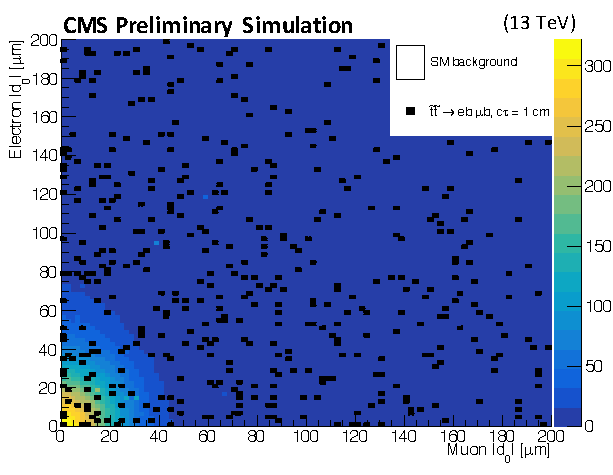
\includegraphics[scale=1.2]{figures/overview/d0_discriminating_power.pdf}
\caption{} 
\label{d0_discriminating_power}
\end{figure}
\fxnote{this is an ugly plot}





% \FIXME: dumping content that didn't make it into other sections
%This transverse impact parameter (\ad) is defined as the distance of closest approach in the transverse plane of the helical trajectory of the lepton track to the center of the luminous region. Another option of a discriminating variable could be the $d_{0}$ significance $\ad/\sigma$, where $\sigma$ is the uncertainty in \ad. However, we choose to simply use \ad) in this analysis because of its straightforward correspondence to the particle lifetime, which makes it an easier variable for theorists to use in their efforts to reinterpret this search. Furthermore, we found that the uncertainty in \ad is often underestimated, which reduces any potential benefit of using $\ad/\sigma$. Figure \ref{fig:signalEventDiagram} shows a diagram of the definition of $d_0$ used in this analysis. The lepton $d_0$ is strongly correlated with the lifetime of the particle from which it decayed. The $d_0$ spectra of leptons from promptly decaying particles, such as top quarks and $\PW$ bosons, will peak at zero and fall sharply. For leptons from particles that travel farther than the resolution of lepton \ad, such as tau leptons and mesons containing bottom or charm quarks, the $d_0$ spectrum will be noticeably wider. For leptons from much longer-lived particles such as the top squarks in the benchmark signal process, the $d_0$ spectrum will be very wide, approaching a flat distribution for the longest top squark lifetimes we consider. The electron and muon \ad distributions are shown for signals at different lifetimes and backgrounds in Fig.\,\ref{fig:PreselectionD0Signal}, for events that pass the $\Pgm\Pgm$ preselection criteria. For a given lifetime, the \ad distributions are the same for the two $\PSQt$ decay modes considered and are independent of $\PSQt$ mass.

% \FIXME: define dz too

\pagebreak